\documentclass{article}
\usepackage{graphicx}
\graphicspath{{images/}}

\title{
    User Manual\\
    \begin{large}
        \textit{Golf Course Mapper}
    \end{large}
}
\date{
    \begin{small}
        \today
    \end{small}
}
\author{
    Team Recursive Recursion \\
    Retro Rabbit
}

\begin{document}
    %===========================================================================
    % TITLE
    %===========================================================================
    \pagenumbering{gobble}
    \maketitle
    \newpage

    %===========================================================================
    % DOCUMENT
    %===========================================================================
    \pagenumbering{arabic}

    
    
	\section{System Overview}    
	\paragraph{}
	The project will allow golf course owners/managers to draw their golf course using the provided web application. While drawing the golf course, details about the map can be added, such as locations of the hole, green, fairway, or any obstacles and hazardous areas.
Golf players will be able to view the map via their Android phones, enabling them to have a hands-on digital map with details of the course. This will allow the user to plan their shots better and more strategically.


	\section{System Configuration}
	 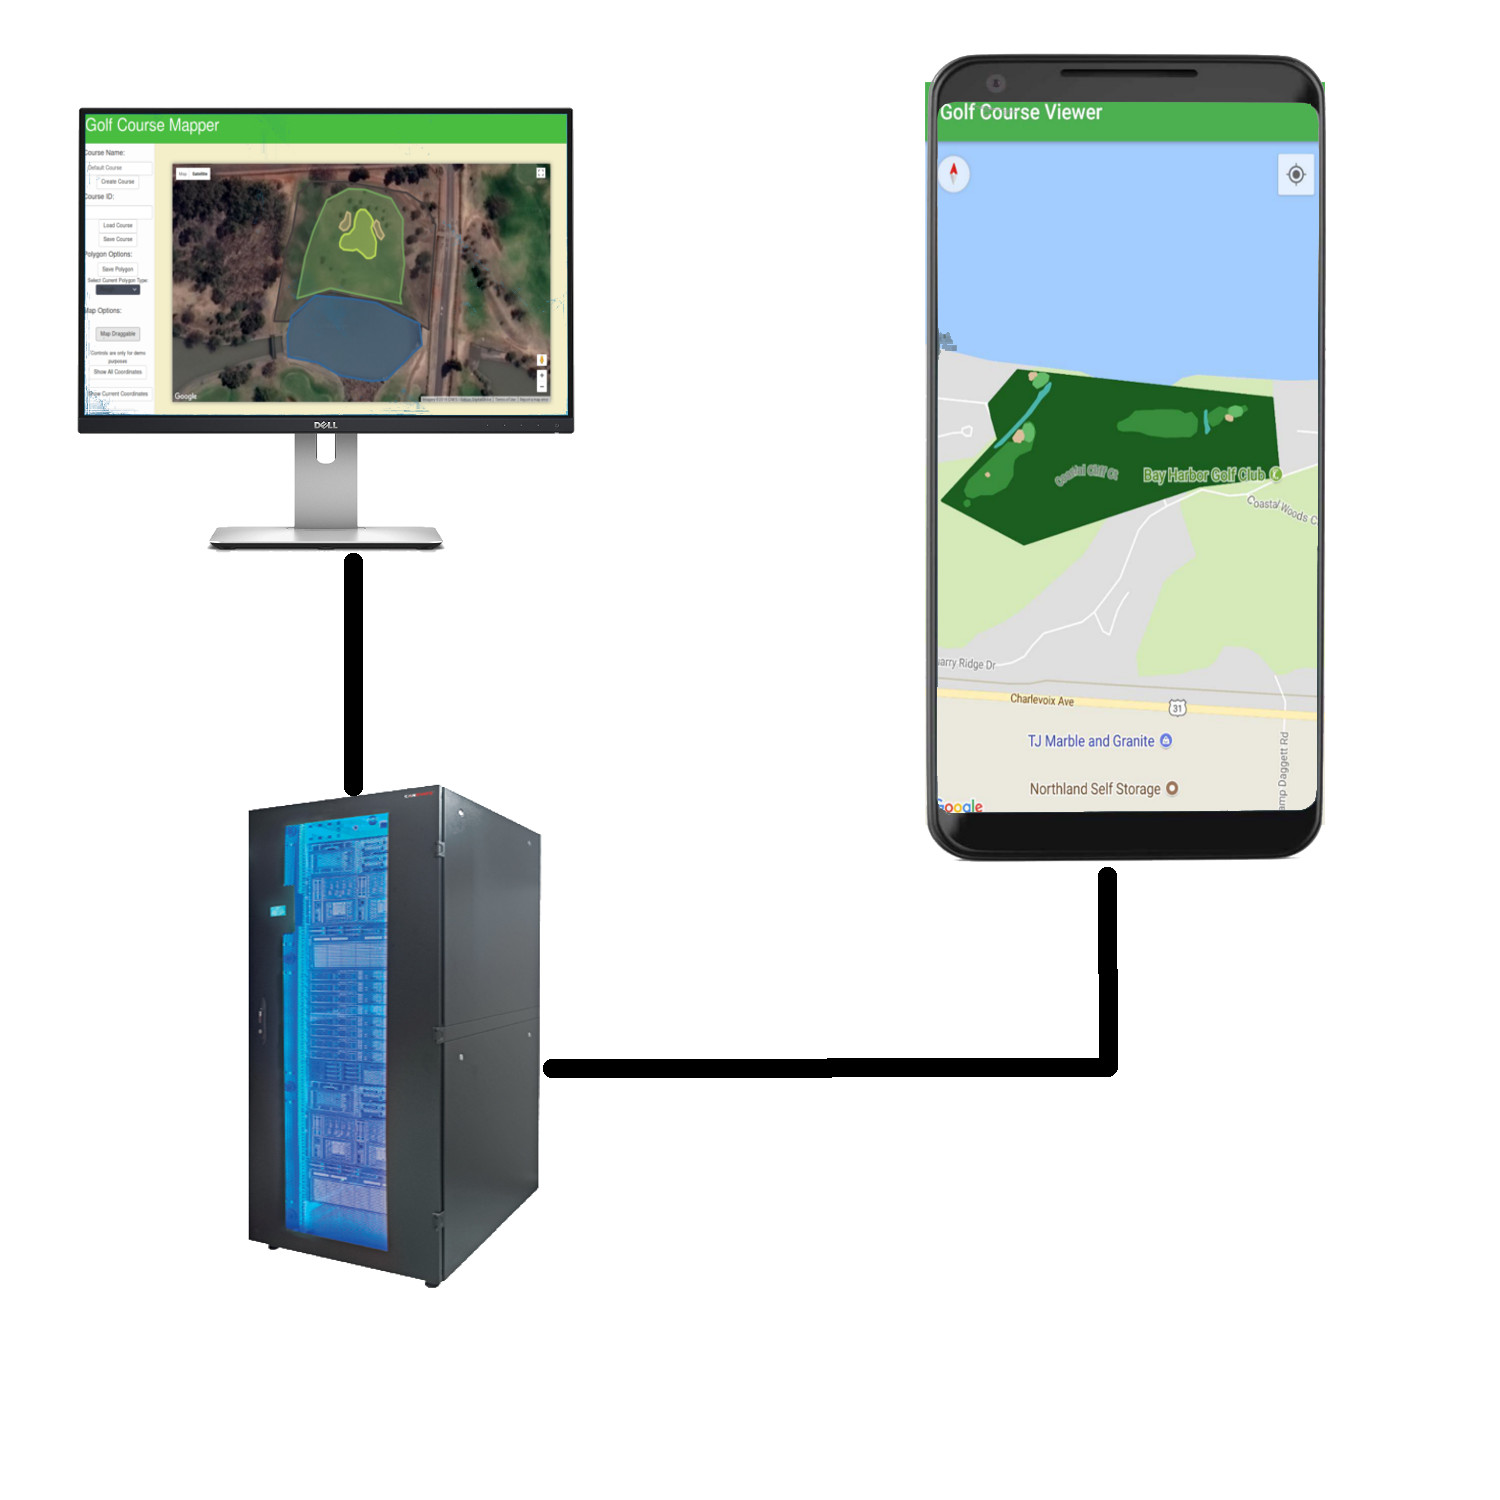
\includegraphics[scale=0.25]{sys-conf-diagram.jpg}
	\paragraph{•}
	  The website and the mobile application connects to the server to retrieve data. An Internet connection is needed to load the map on both the web and mobile application. It is recommended to have Android 4.4 or later for the mobile application. The latest version of Internet Explorer, Google Chrome or Mozilla Firefox is recommended.
	
	\section{Getting Started}
	\paragraph{•}
	
	Website: To access the website go to the URL (http://localhost:5000/).If this is your first time using the website, please register your credentials. If you have used the website before login with your credential that you used to register. 
	
	Mobile Application: To access the mobile application press on the application on a mobile device.
	\section{Using the System}
	
	\subsection{Register and Login}
	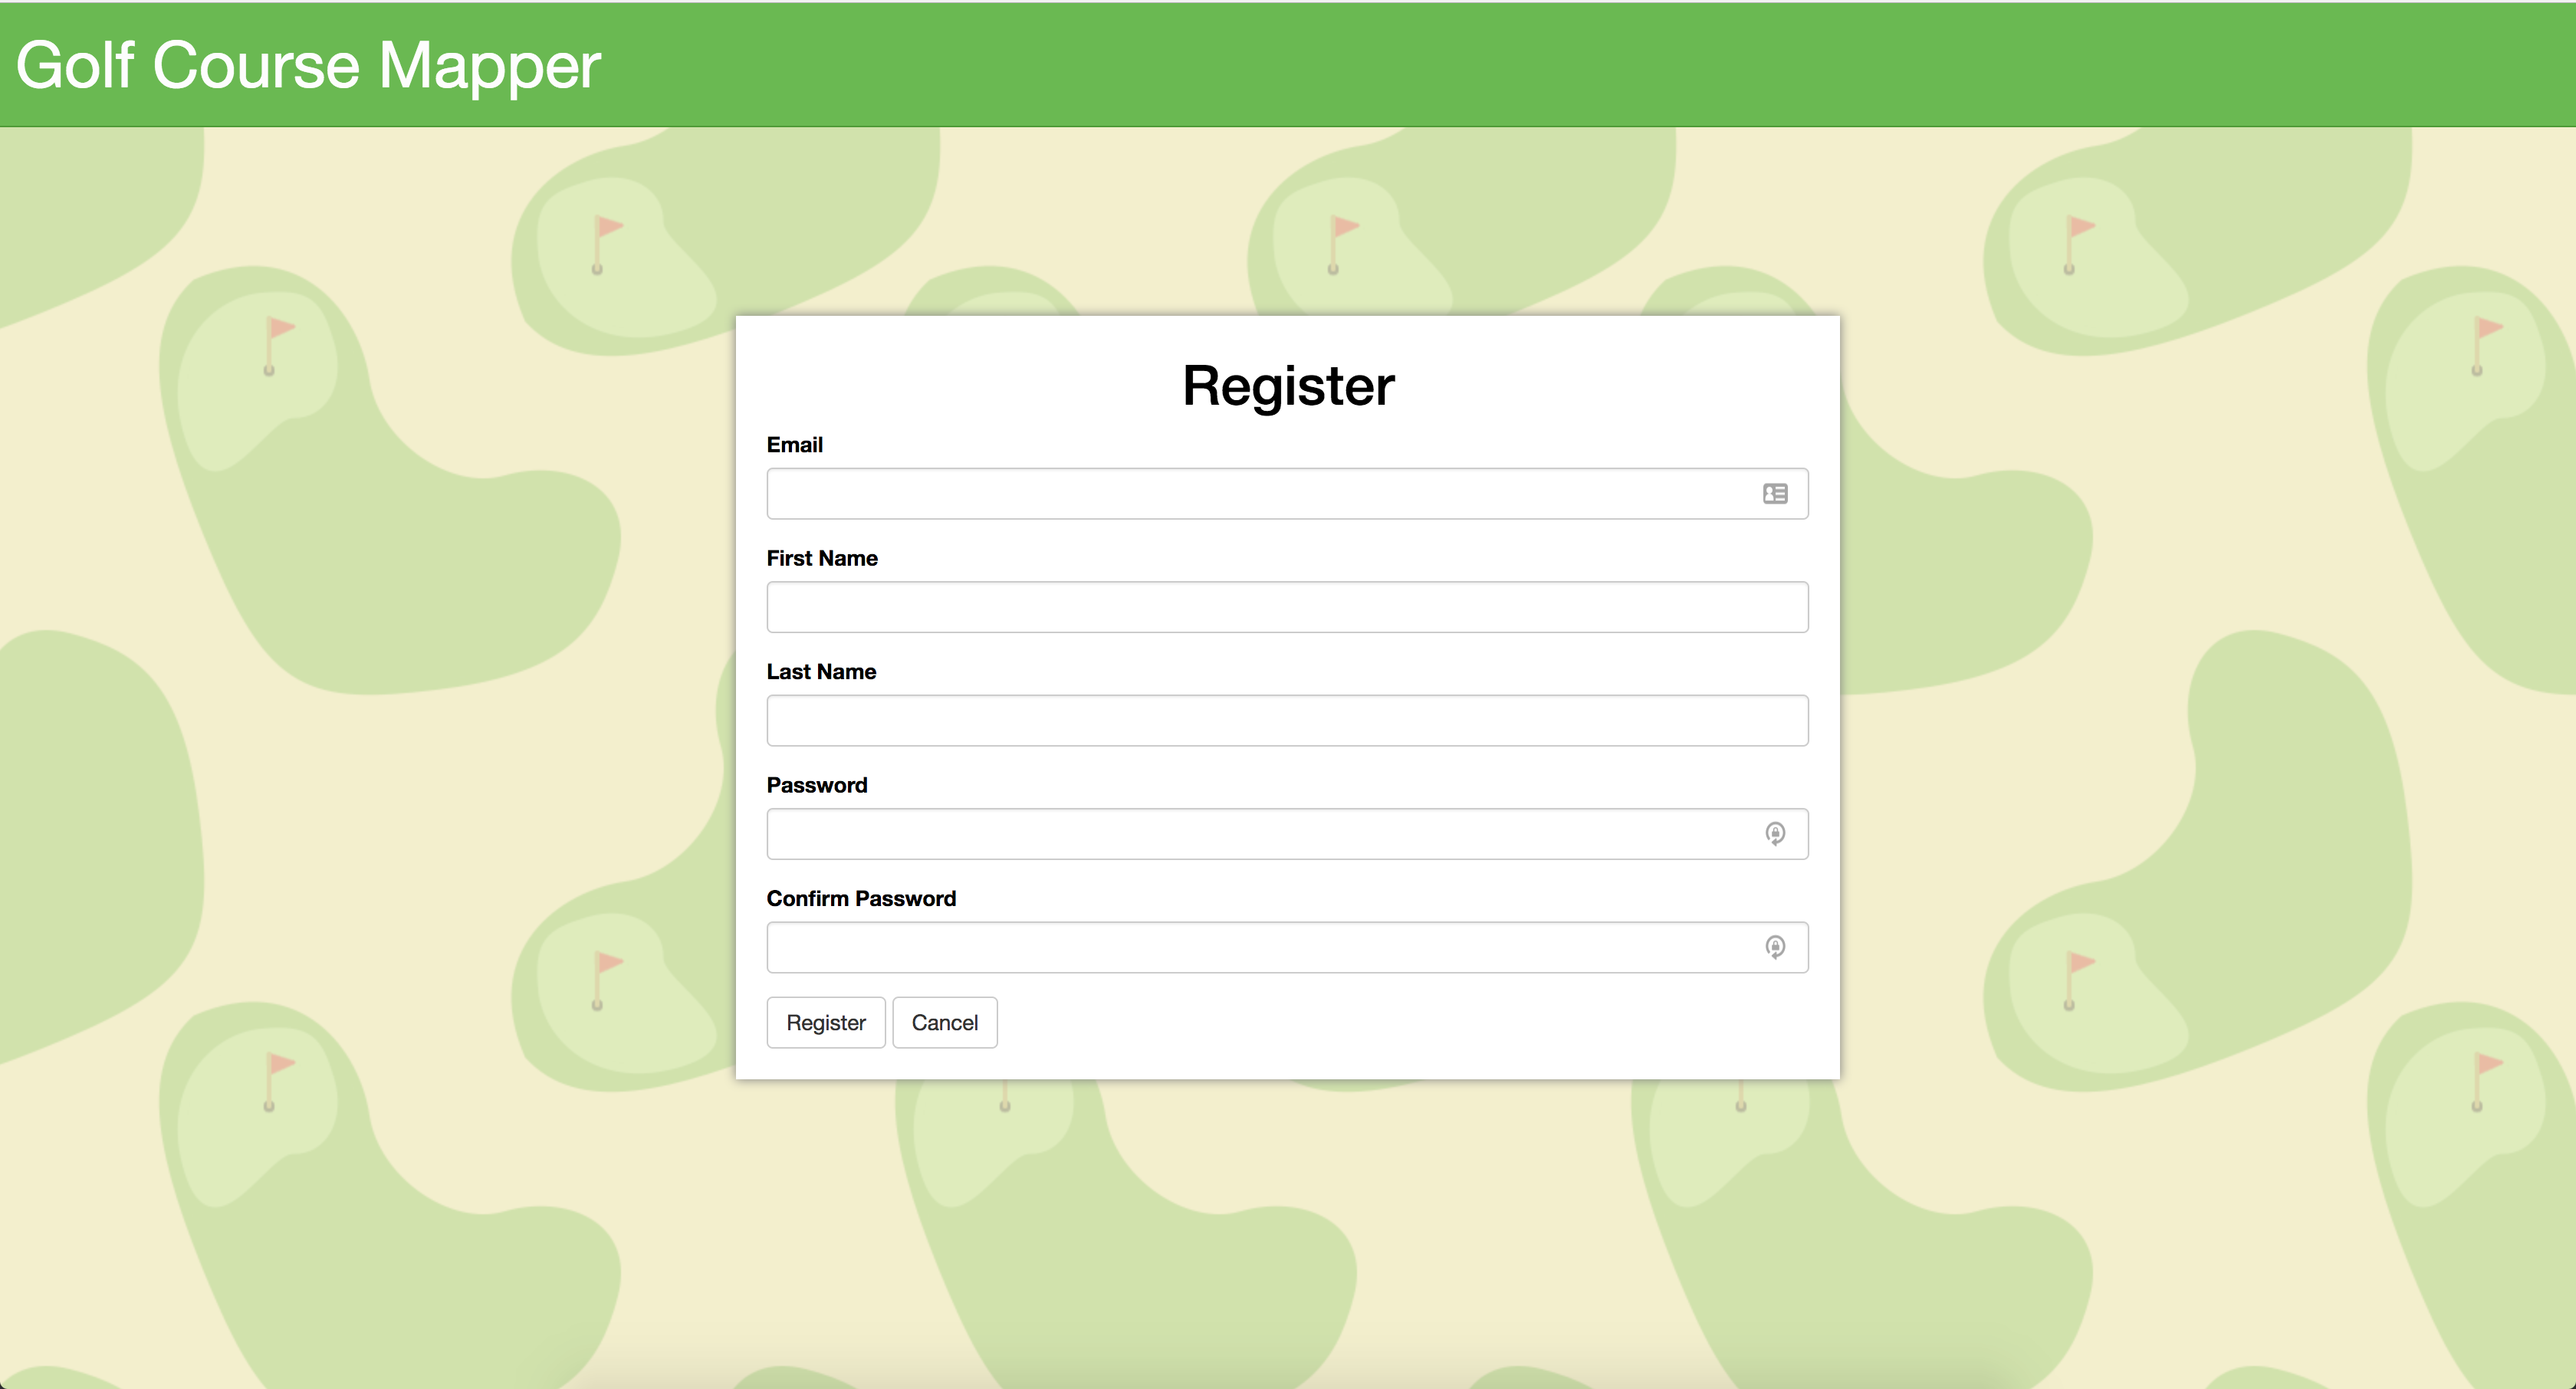
\includegraphics[scale=0.25]{Register}
	\paragraph{•}
    Figure 1.
	\subsubsection{Register}
	\paragraph{•}
	To register for the website, type in your credentials in the text boxes as seen in figure 1. The fields are Email, First Name, Last Name, Password and Confirm Password. After your details have been entered, click on the Register button to register.
	
		
	
	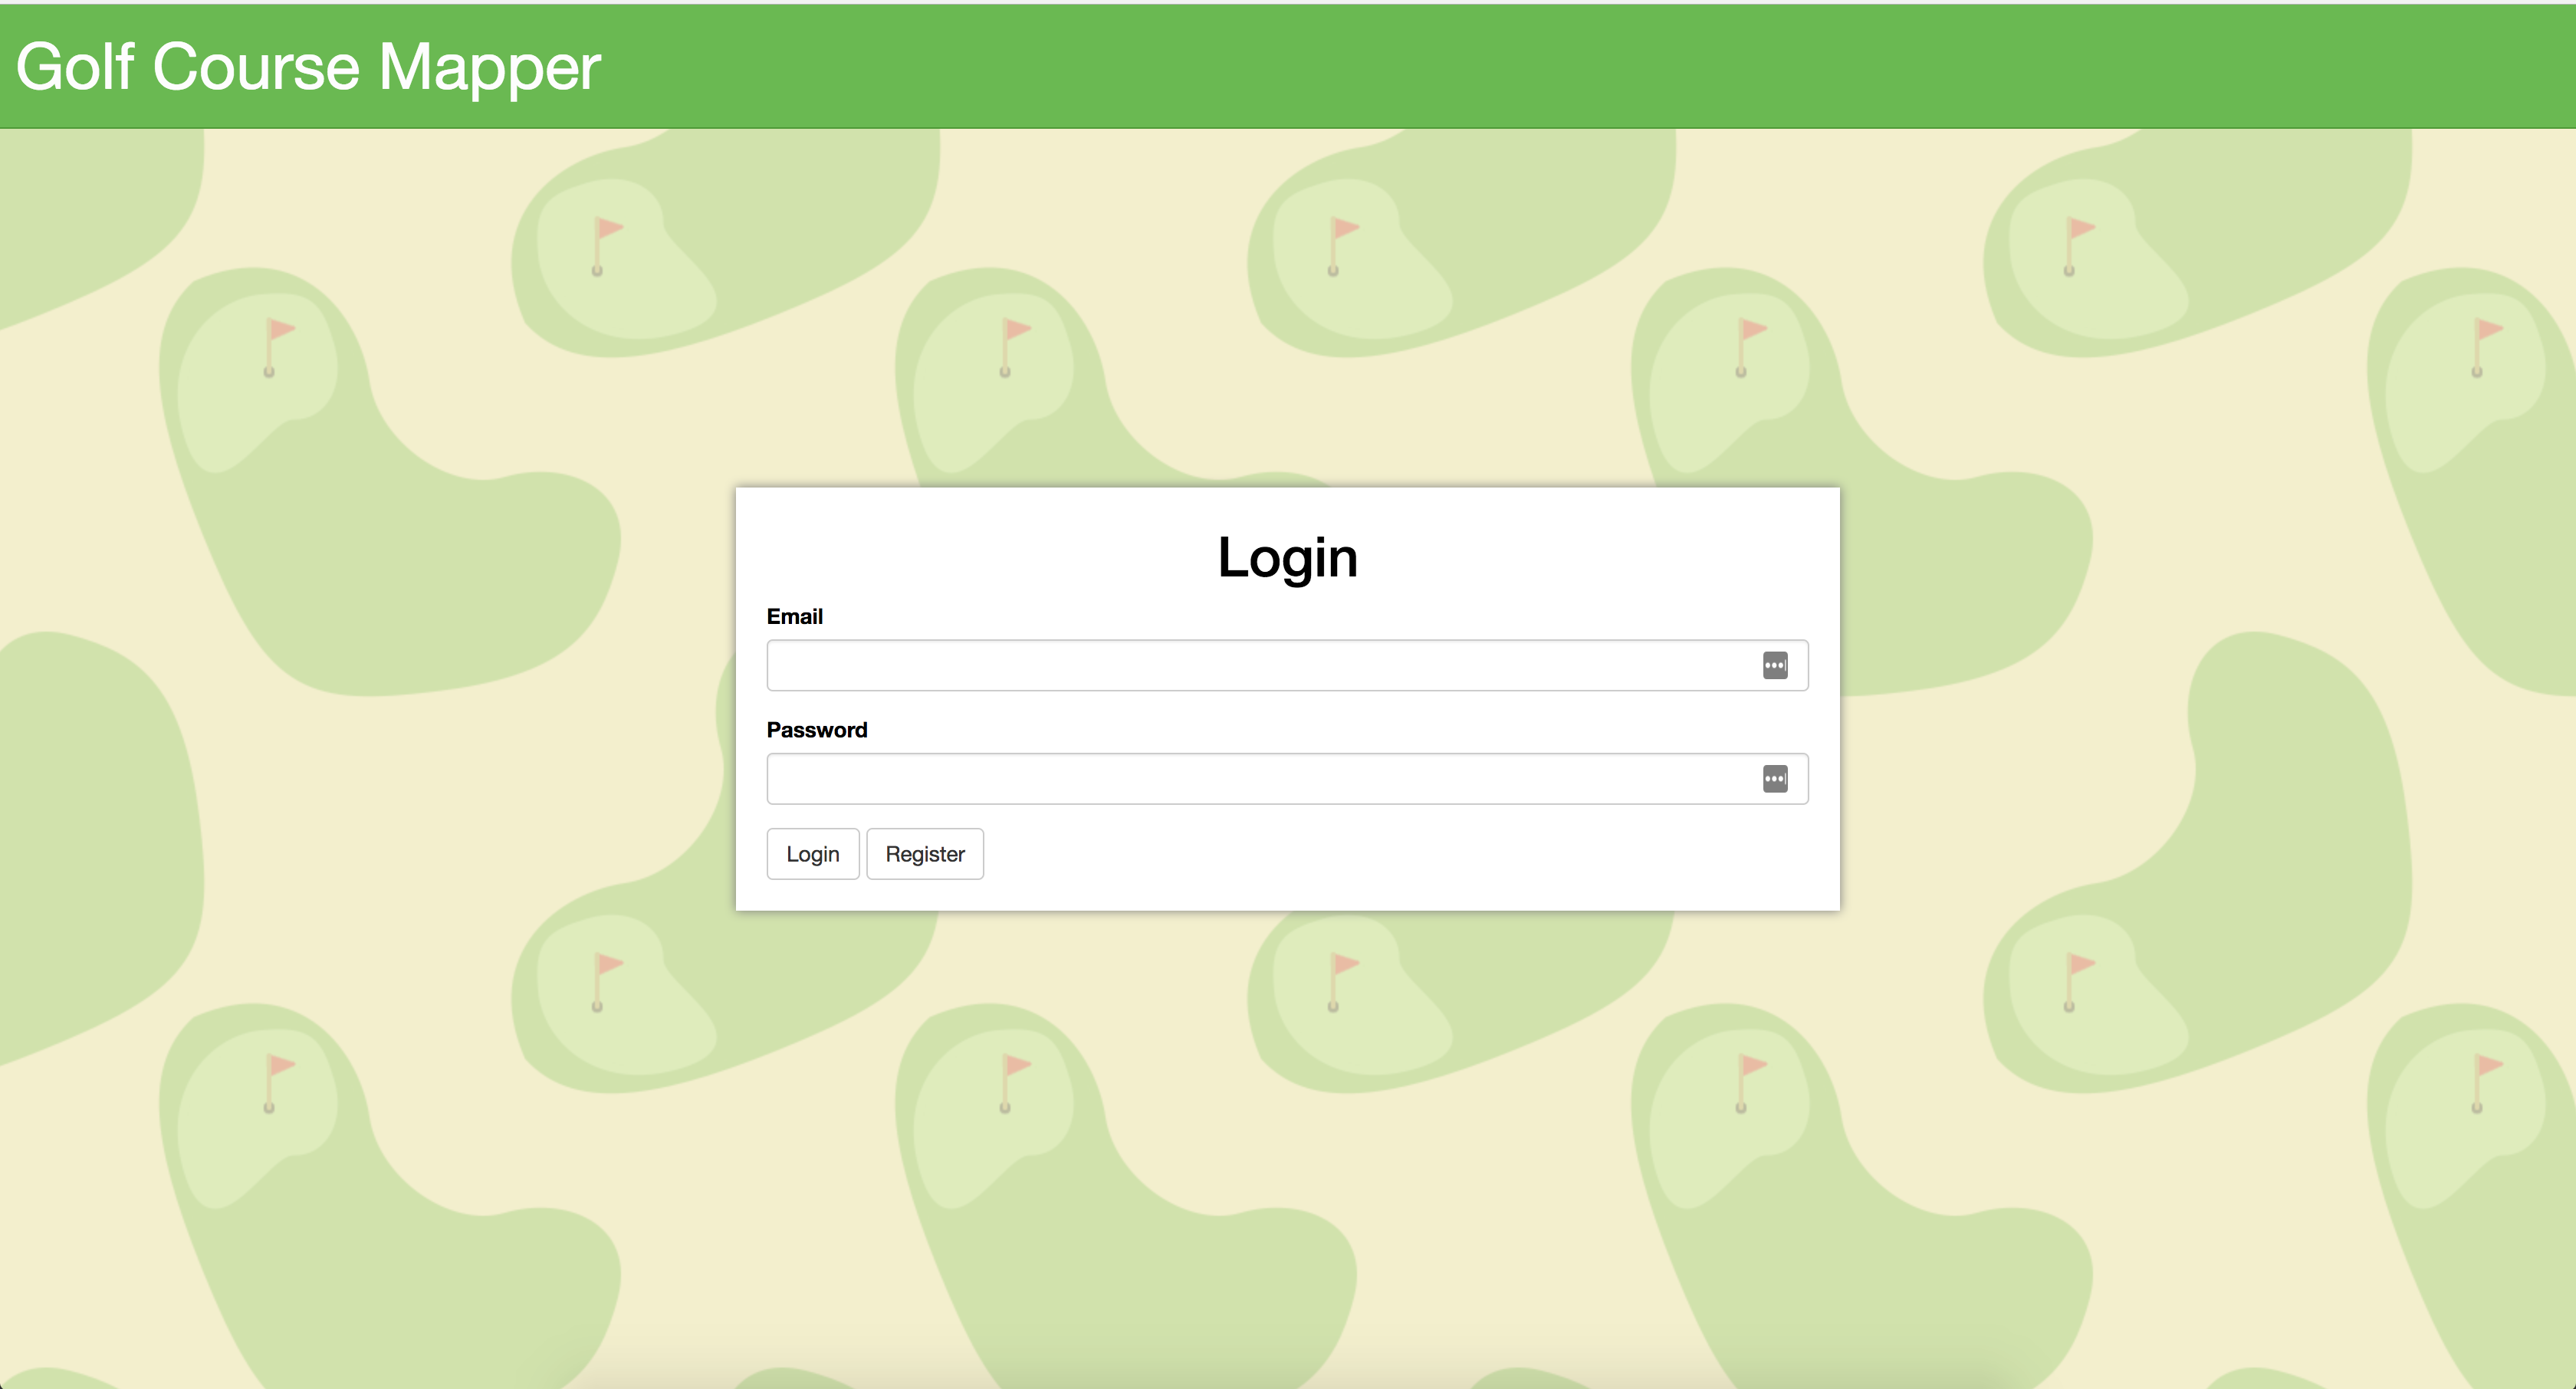
\includegraphics[scale=0.25]{Login}
	\paragraph{•}
    Figure 2.
	\subsubsection{Login}
	\paragraph{•}
	After you have successfully registered your credentials (see 4.1 for more details). Type in the same Email and Password that you registered with, click on the Login button to login. As seen in figure 2.
	
    \subsection{Website}
    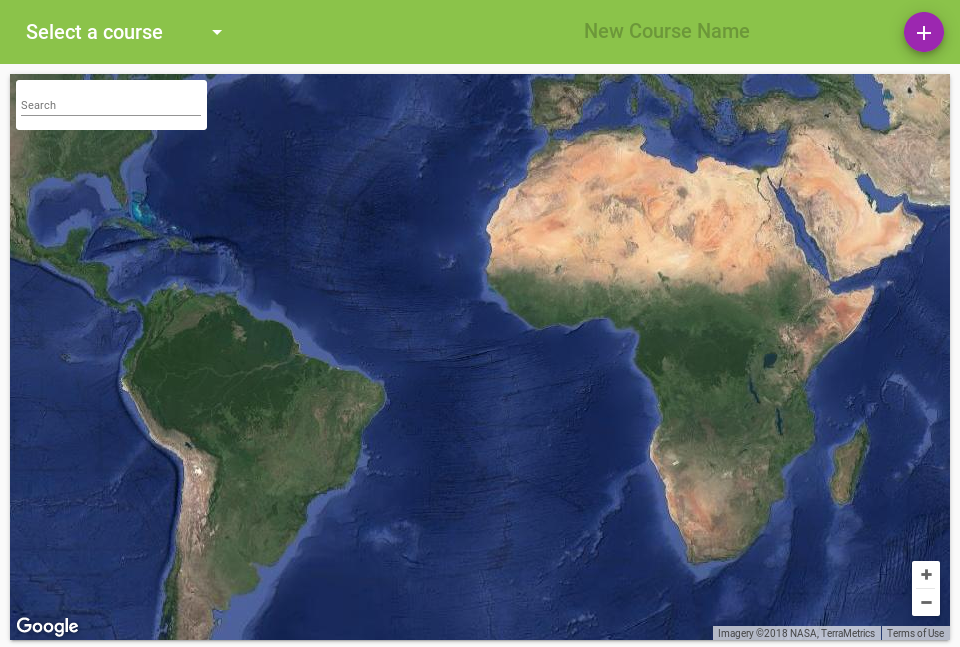
\includegraphics[scale=0.4]{map}
    \paragraph{•}
    Figure 3.
    
	\subsubsection{Select a Golf Course}    
	\paragraph{•}    
	To select a course click on the "Select a course" text as shown in Figure 3. A drop down menu will appear with all the available course. Click on the desired course to load the course onto the map.    
    
    
    \subsubsection{Create Golf Course}
    \paragraph{•}
    Type in the name in the "New Course Name" of the desired golf course to create the course as shown in Figure 3. After a appropriate name has been chosen, click on the "+" button. The course will now be created with the chosen name.
	
	\subsubsection{Search Golf Course}
	\paragraph{•}    
    Type in a name of a location to search it on the map.
    
    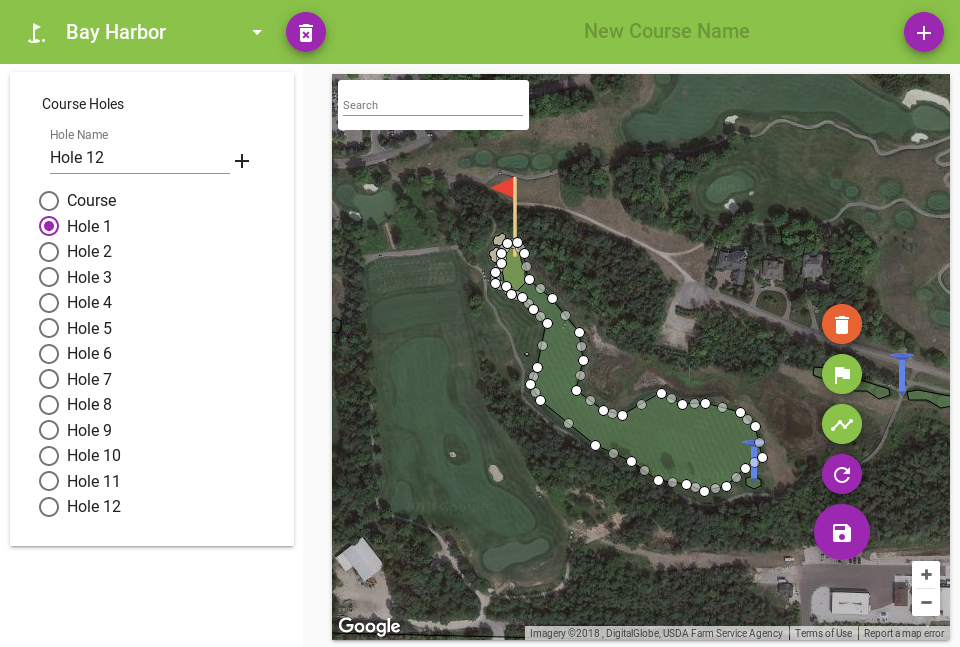
\includegraphics[scale=0.4]{map1}
    \paragraph{•}
    Figure 4
    
    \subsubsection{Create a Hole}
    \paragraph{•}
    Type in the name of the hole in the "Hole Name" text box. Click on the "+" icon to create the hole.
    
    \subsubsection{Select a Hole}
    \paragraph{•}
    To select a hole click on the circle icon next to the desired hole to select and view the hole on the map.
    
    \subsubsection{Delete an Element}
    \paragraph{•}
    To delete an element click on the element and then click on the red trash can icon. The selected element will now be deleted.
    
    \subsubsection{Place a Marker}
	\paragraph{•}
	To place a marker on the map, click on the green flag icon on the right of the screen. Click on a desired location for the marker to be placed. A menu will appear to select the type of marker and to add additional information. Click on the done button to finish the marker placing. The available markers are: Hole, Tee, and Pin
	
	\subsubsection{Polygon}
    \paragraph{}
    To create a polygon or map out a element, click on the green line icon. To create the polygon click on the map in the desired locations. Lines will appear as the user click, when the polygon has been completed a menu will appear to choose the element type. The available types are: Green, Fairway, Water hazard, and sand bunker.
    
	\subsubsection{Reload Course}    
	\paragraph{•}
	To reload the course, click on the purple reload icon on the right of the screen. The map will now reload.
	
    
    \subsubsection{Save Course} 
    \paragraph{}
    To save changes made to a course or hole, click on the purple save icon on the right of the screen. Any changes made will now be saved.
    
    \subsubsection{Delete Course}
	\paragraph{•} 
	To delete a course, load the desired course. Click on the purple trash can on the right of the course name to delete the golf course.


	\subsection{Mobile Application}
	    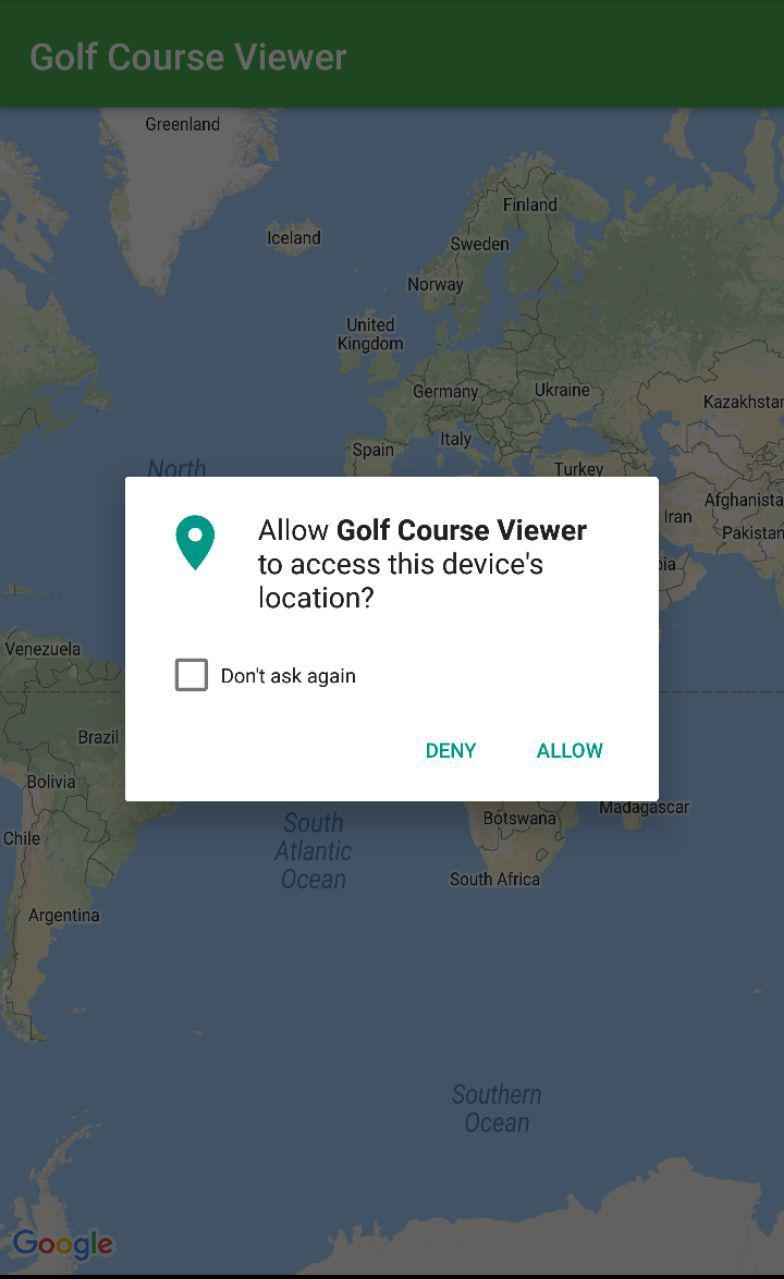
\includegraphics[scale=0.2]{mobileapp-permissions.jpg}
	    \linebreak
	    Figure 5
	\subsubsection{Allow Permissions}
	
	\paragraph{•}
	When starting the application, a message will pop up to ask for permissions to use location services. Press "Allow" to allow location services to be used.
	
	\subsubsection{View Course}
	    \includegraphics[scale=0.8]{coursemap.png}
	    Figure 6
	
	\paragraph{•}
	Move around by touching and zoom by pinching the screen. Move to the location of gold course created to view the course. The next hole can be seen by tapping on the blue arrow on the right button
	
	\subsubsection{Select Course}
	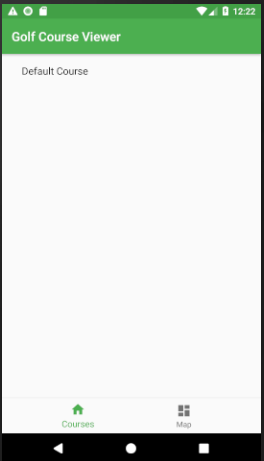
\includegraphics[scale=0.7]{CourseListUI.PNG}
	\linebreak
	Figure 7
	
	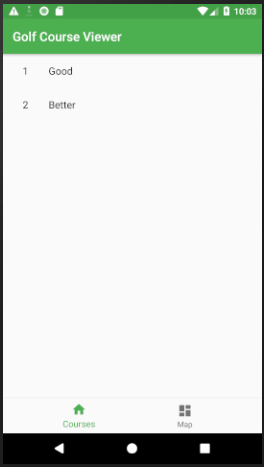
\includegraphics[scale=0.7]{Holes.PNG}
	\linebreak
	Figure 8
	
	
	\paragraph{•}
	Press on the Courses item in the bottom navigation bar to view to available courses as shown in Figure 7. Press on the desired course to view the course. After the course has been chosen, the hole can then be selected as shown in Figure 8
	
	

	
	
\end{document}